\documentclass[12pt]{article}
\pdfoutput=1

\usepackage[T1]{fontenc}
%\usepackage[latin9]{inputenc}
\usepackage{verbatim}
\usepackage{float}
\usepackage{amsthm}
\usepackage{amsmath}
\usepackage{amssymb}
\usepackage{graphicx}
%\usepackage{multirow}
\usepackage{color}
\usepackage{url}
\usepackage{caption}
\usepackage{subcaption}
\usepackage{mathtools} 
\usepackage{stackrel} 
%\usepackage[skip=1pt]{caption} % example skip set to 2pt


\newcommand{\LL}{\mathcal{L}}
\newcommand{\E}{\mathbb{E}}
\newcommand{\I}{\mathcal{I}}
\newcommand{\ep}{\varepsilon}
\newcommand{\Z}{\mathbb{Z}}
\newcommand{\GCD}{\mathbf{GCD}}
\newcommand{\XX}{\mathcal{X}}
\newcommand{\SUM}{\text{sum}}
\newcommand{\1}{\mathbf{1}}
\newcommand{\rr}{\textbf{r}}
\newcommand{\ii}{\textbf{i}}
\newcommand{\jj}{\textbf{j}}

\newcommand{\II}{\mathcal{I}}
\newcommand{\kk}{\textbf{k}}
\newcommand{\RR}{\mathbb{R}}
\newcommand{\mb}{\mathbf}
\newcommand{\mk}{\mathfrak}
\newcommand{\mc}{\mathcal}
\newcommand*\Bell{\ensuremath{\boldsymbol\ell}}
\newcommand{\TODO}[1]{{\color{red}{[#1]}}}
\newcommand{\revised}[1]{{\color{blue}{#1}}}

%\newcommand{\SNR}{\ensuremath{\textsf{SNR}}}
\makeatletter

\newcommand{\reals}{\mathbb{R}}
\newcommand{\RL}{\mathbb{R}^L}
\newcommand{\tamir}{x}
\newcommand{\CL}{\mathbb{C}^L}
\newcommand{\RN}{\mathbb{R}^N}
\newcommand{\RNN}{\mathbb{R}^{N\times N}}
\newcommand{\RPP}{\mathbb{R}^{P\times P}}
\newcommand{\CNN}{\mathbb{C}^{N\times N}}
\newcommand{\inner}[1]{\left\langle {#1} \right\rangle}
\newcommand{\hx}{\hat{x}} 
\newcommand{\one}{\mathbf{1}} 
\newcommand{\be}
{\begin{equation}}
\newcommand{\ee}
{\end{equation}}
%\renewcommand{\P}{\mathbb{P}}
\newcommand{\aseq}{\stackrel{a.s.}{=}}
\renewcommand{\P}{\mathrm{Prob}}


\theoremstyle{plain}
\newtheorem{thm}{\protect\theoremname}[section]
\theoremstyle{definition}
\newtheorem{defn}[thm]{\protect\definitionname}
\theoremstyle{remark}
\newtheorem{claim}[thm]{\protect\claimname}
\theoremstyle{plain}
\newtheorem{lem}[thm]{\protect\lemmaname}
\newtheorem*{lem*}{Lemma}
\theoremstyle{remark}
\newtheorem{rem}[thm]{\protect\remarkname}
\theoremstyle{plain}
\newtheorem{corollary}[thm]{\protect\corollaryname}
\theoremstyle{plain}
\newtheorem{proposition}[thm]{\protect\propositionname}
\providecommand{\claimname}{Claim}
\providecommand{\definitionname}{Definition}
\providecommand{\lemmaname}{Lemma}
\providecommand{\remarkname}{Remark}
\providecommand{\theoremname}{Theorem}
\providecommand{\corollaryname}{Corollary}
\providecommand{\propositionname}{Proposition}

\usepackage{authblk}
\renewcommand*{\Affilfont}{\normalsize}
\setlength{\affilsep}{2em}   % set the space between author and affiliation

\usepackage[margin=.6in]{geometry}

\newenvironment{myquote}[1]%
{\list{}{\leftmargin=#1\rightmargin=#1}\item[]}%
{\endlist}

\allowdisplaybreaks


\begin{document}

%\begin{frontmatter}


\title{TBD}
%
%\author[a]{Tamir Bendory}
%\author[b]{Nicolas Boumal} 
%\author[c]{William Leeb}
%\author[a,b]{Eitan Levin}
%\author[a,b]{Amit Singer}
%
%\affil[a]{The Program in Applied and Computational Mathematics, Princeton University, Princeton, NJ, USA}
%\affil[b]{Department of Mathematics, Princeton University, Princeton, NJ, USA}
%\affil[c]{School of Mathematics, University of
%	Minnesota, Minneapolis, MN, USA }

%\date{}
\maketitle



\begin{abstract}
abstract
%Single-particle cryo-electron microscopy (cryo-EM) has recently joined X-ray crystallography
%and NMR spectroscopy as a high-resolution structural method for biological macromolecules.
%In a cryo-EM experiment, the microscope produces images called micrographs. Projections of the molecule of interest are embedded in the micrographs at unknown locations, and under unknown viewing directions. Standard imaging techniques first locate these projections (detection) and then reconstruct the 3-D structure from them. Unfortunately, high noise levels hinder detection. When reliable detection is rendered impossible, the standard techniques fail. This is a problem especially for small molecules, which can be particularly hard to detect. In this paper, we propose a radically different approach: we contend that the structure could, in principle, be reconstructed directly from the micrographs, without intermediate detection. 
%As a result, even small molecules should be within reach for cryo-EM. To support this claim, we setup a simplified mathematical model and demonstrate how our autocorrelation analysis technique allows to go directly from the micrographs to the sought signals. This involves only one pass over the micrographs, which is desirable for large experiments. 
%We show numerical results and  discuss challenges that lay ahead to turn this proof-of-concept into a competitive alternative to state-of-the-art algorithms.
\end{abstract}

\section{Introduction}

\subsection{Model}

In this paper, we consider the problem of recovering signals that appear 
multiple times at unknown locations in a noisy measurement. This problem can be conveniently posed as  \emph{blind deconvolution}.
Let $x\in\RL$ be the sought signal and let $y\in\RN$ be the observed data, where we assume $N$ is  far larger than $L$. Let  $s \in \{0, 1\}^{N-L+1}$ be a binary signal indicating (with 1's) the starting positions of all occurrences of $x$ in $y$, so that, with additive white Gaussian noise:
\begin{equation} 
y  =  x \ast s + \varepsilon, \quad  \varepsilon   \sim \mathcal{N}(0,\sigma^2 I_N),
\label{eq:model}
\end{equation}
where $\ast$ denotes linear convolution. 
While both $x$ and $s$ are unknown, the goal is only to estimate $x$ from $y$. 
We refer to~\eqref{eq:model} as the \emph{homogeneous model}.
This is a key difference with other works on  \emph{blind deconvolution}, a longstanding problem arising in a variety of engineering and scientific applications such as astronomy, communication, image deblurring, system identification and optics; see~\cite{jefferies1993restoration,shalvi1990new,ayers1988iterative,abed1997blind}, just to name a few. 
The parameters of the signal $s$ (the locations of its nonzero values) are the \emph{nuisance variables} of the problem. As will be shown next, in a low SNR environment, estimating $s$ is impossible, whereas estimating $x$ is tractable under some conditions on $s$. 
This model appears in several scientific applications, including spike sorting~\cite{lewicki1998review}, passive radar~\cite{gogineni2017passive} and system identification~\cite{ljung1998system}

We also consider a natural generalization, called the \emph{heterogeneous model}, in which one aims to estimate a set of $K$ signals $x_1,\ldots,x_K\in\RL$ from their mixed blind deconvolution
\begin{equation} 
y  =  \sum_{i=1}^Kx_i \ast s_i + \varepsilon, \quad  \varepsilon   \sim \mathcal{N}(0,\sigma^2 I_N),
\label{eq:model}
\end{equation}
where again $s_i$ denotes a binary signal. 

The signals $s_i$ indicate the support of the occurrences of $x$ in the data. We will consider two generative models for $s$: well-spaced deterministic model, and a stochastic Possion model.

\paragraph{Well-separated support model:} In this model, 
we assume the binary signal $s$ obeys \TODO{This is not accurate}
\begin{equation}
\textrm{If } s[i] = 1 \textrm{ and } s[j] = 1 \textrm{ for } i \neq j, \textrm{ then } |i - j| \geq 2L-1.
\label{eq:spacing}
\end{equation}
In words: the starting positions of any two occurrences  must be separated by at least $2L-1$ positions, so that their end points are necessarily separated by at least $L-1$ signal-free entries in the data.
%
\paragraph{Poisson support model:}

The relation between the two models is formulated in Section~\ref{sec:support}.

In order to recover the image, we use autocorrelation analysis. Specifically, we relate the autocorrelations of the micrographs to the autocorrelations of the image.
For any noise level, these autocorrelations can be estimated to any desired accuracy, provided that we  observe sufficiently many image occurrences and the latter are separated in the micrograph. Importantly, there is no need to detect individual image occurrences. The autocorrelations of the micrographs are straightforward to compute and require only one pass over the data. After estimation of the density of particles in the micrographs, these directly yield estimates for the autocorrelations of the target image itself. To estimate the image itself from its estimated autocorrelations, we solve a nonlinear inverse problem

\subsection{Main motivation: single-particle reconstruction using cryo-electron microscopy}
This work is motivated by the problem of single-particle reconstruction using cryo-electron microscopy (cryo-EM).  Cryo-EM is revolutionizing the field of structural biology, enabling XXX. 

In a cryo--EM experiment, biological samples are rapidly frozen in a thin layer of vitreous ice.
The microscope produces a 2-D tomographic image of the samples embedded in the ice, called a \emph{micrograph}. Each micrograph contains tomographic projections of the samples at unknown locations and under unknown viewing directions. The goal is to construct 3-D models of the molecular structure from the micrographs.

The signal to noise ratio (SNR) of the projections in the micrographs is a function of two dominating factors. On the one hand, the SNR is a function of the electron dose. To keep radiation damage within acceptable bounds, the dose must be kept low, which leads to high noise levels. On the other hand, the SNR is a function of the molecule size. The smaller the molecules, the fewer detected electrons carry information about them.


All contemporary methods in the field split the reconstruction procedure into two main  stages.
The first stage consists in extracting the various particle projections from the micrographs. This stage is called \emph{particle picking}. The second stage aims to construct a 3-D model of the molecular structure from these projections. The quality of the reconstruction eventually hinges on the quality of the particle picking stage.
Crucially, it can be shown that reliable detection of individual particles is impossible below a certain critical SNR. This fact has been recognized early on by the cryo-EM community. In particular, in an influential paper from 1995, Richard Henderson~\cite{henderson1995limitations} investigates the following 
In that paper and in others that followed (e.g.,~\cite{glaeser1999electron}), it was established that particle picking is impossible for molecules below a certain weight (below $\sim$50 kDa). 

As these two leaders of the cryo-EM community point out, it is impossible to reconstruct small molecules by any of the existing computational pipelines for single particle analysis in cryo--EM, because the particles themselves cannot be picked from the micrographs. Yet, imaging such molecules is important for structure-guided drug design and other applications~\cite{scapin2018cryo}.



The unique issues raised by small particles have been mitigated by recent technological advances in the field, including the use of Volta phase plates~\cite{khoshouei2017cryo,liang2017phase} and scaffolding cages~\cite{liu2018nearatomic}.
Despite this progress, detecting small molecules in the micrographs remains a challenge.
We note that nuclear magnetic resonance (NMR) spectroscopy and X-ray crystallography are well suited to reconstruct small molecules. Yet, cryo--EM has a lot to offer even for molecules with already known structures obtained via NMR spectroscopy or X-ray crystallography, because these methods have limited ability to distinguish conformational variability.  

In a recent paper~\cite{bendory2018toward} by the authors, it was suggested to bypass the particle picking stage and the reconstruct the 3-D structure directly from the micrograph.
In that paper, we have shown that, at least in principle, the limits particle picking imposes on molecule size do not necessarily  translate into limits on particle reconstruction.
The principle mathematical tool is the method of moments, or autocorrelation analysis, described in Section~\ref{sec:AC_analysis}.

This goal of  this paper is to provide a theoretical and numerical justification for the method proposed in~\cite{bendory2018toward}.  
In particular, the homogeneous  model serves as an abstraction of the cryo-EM problem. While in cryo-EM the 2-D images are tomographic projections of a 3-D structure, taken from unknown viewing directions, in the homogeneous model we observe the same 2-D image again and again. The heterogeneous case generalizes to multiple signals. 

To talk about the MRA-Kam's method relations. Also, model bias 
\TODO{Where do we discuss the limits of detection?}
%
%Beyond this 2-D proof of concept, we look toward \mbox{3-D} reconstruction as well. Zvi Kam~\cite{kam1980reconstruction} first proposed autocorrelation analysis for \mbox{3-D} reconstruction, under the assumption of perfect particle picking: his method used autocorrelations of the picked, perfectly centered, particles. In contrast, we derive the mathematical relation between the autocorrelations of the micrographs as a whole and the \mbox{3-D} volume, under some simplifying conditions.
%We show a few numerical examples and outline the future developments required to make this method applicable to experimental  data. 
%
%Another interesting feature of the described approach pertains to model bias, whose importance in cryo-EM was stressed by a number of authors~\cite{shatsky2009method,vanheel1992correlation,henderson2013avoiding,vanheel2013finding}. In the classical ``Einstein from noise'' experiment, multiple realizations of pure noise are aligned to a picture of Einstein using template matching and then averaged. In~\cite{shatsky2009method}, it was shown that the averaged noise rapidly becomes remarkably similar to the Einstein template. In the context of cryo--EM, this experiment exemplifies how prior assumptions about the particles may influence the reconstructed structure. This model bias is common to all particle picking methods based on template matching. In our approach, no templates or human intervention are required, thus significantly reducing concerns about model bias. %


%Our problem can be interpreted as a special case of the \emph{system identification} problem. Similarly to~\eqref{eq:model}, the
%forward model takes the form
%%
%\begin{math}
%%
%y = x\ast w + \varepsilon,  
%%
%\end{math} 
%%
%where $x$ is the unknown signal (the system's impulse response), $w$ is an unknown (often random) input sequence, and $\varepsilon$ is an additive noise.
%The goal of this problem is to estimate $x$, usually referred to as ``identifying the system.'' The question of identifiability of $x$ under this observation model is addressed for certain Gaussian and non-Gaussian $w$ in~\cite{benveniste1980robust,kormylo1983identifiability}. In the special case where $w$ is binary and satisfies our separation condition, we recover our model. 
%
%Likelihood-based methods estimate $x$ as the maximizer of some function $f(x | y)$, where $f$ is derived from the likelihood function of $x$ given the observed signal $y$.  
%If some prior is assumed on $x$, then $f(x|y)$ can be taken to be the posterior distribution of $x$ given the data; this is the simplest form of Bayesian inference.
%Methods based on such formulations are popular nowadays in cryo-EM; see for instance~\cite{sigworth1998maximum,scheres2012relion}. 
%Optimizing the function $f(x|y)$ exactly is often intractable, and thus heuristic methods are used instead. One proposed technique is to use Markov Chain Monte Carlo (MCMC)~\cite{cappe1999simulation}. 
%In special cases, including the case where $w$ is binary, expectation maximization (EM) has been used~\cite{cappe1999simulation}. The EM method for discrete $w$ is based on a certain ``forward-backward'' procedure used in hidden Markov models~\cite{rabiner1989tutorial}. However, the complexity of this procedure is superlinear in $N$, and therefore its usage is limited for big data sets. 
%
%Because likelihood methods are computationally expensive, methods based on recovery from moments have also been previously used for system identification. Methods based on the third- and fourth-order moments are described and analyzed in~\cite{lii1982deconvolution,giannakis1989identification,tugnait1984identification}. Building on such ideas, we focus on an autocorrelation analysis for~\eqref{eq:model}. 


%
%\section{The detection limit} \label{sec:detectionlimit}
%
%In the low SNR regime---even if $x$ is known---estimating the binary sparse signal $s$ is impossible, that is, one cannot reliably detect occurrences of $x$ in the micrograph $y$.
%To support this claim, we consider a strictly simpler problem: suppose an oracle identifies for us one interval of length $L$ in the micrograph that either contains a full signal occurrence (plus noise), or contains just noise. Our task is to determine which one it is, that is, to determine whether the corresponding entry of $s$ is 0 or 1.
%The oracle further provides the signal $x$, the probability $q$ that  the interval contains signal, and the noise variance $\sigma^2$. 
%
%This decision problem can be abstracted as follows: We have two known vectors $\theta_0 = x$ and $\theta_1 = 0$ in $\mathbb{R}^L$. There is a random variable $\eta$ taking values 0 or 1 with probabilities $q$ and $1-q$, respectively. We observe a random vector $X \in \mathbb{R}^L$ (an extract of the micrograph) with the following distribution: if $\eta = 0$, then $X \sim \mathcal N(\theta_0,\sigma^2I_L)$ and if $\eta = 1$, then $X \sim \mathcal N(\theta_1,\sigma^2I_L)$. 
%
%We observe $X$, and our task is to estimate $\eta$. How reliably can this be done? If $q \geq 1/2$, the constant estimator $\hat{\eta} = 0$ is correct with probability $q$; likewise, if $q \leq 1/2$, the constant estimator $\hat{\eta} = 1$ is correct with probability $1-q$. The question is, can we do better than this?  We prove that, as $\sigma \to \infty$, the answer is no. The result is proved in Appendix~\ref{sec:proof_two_gauss}.
%
%\begin{proposition} \label{prop:two_gauss}
%	For any deterministic estimator $\hat{\eta }$ of $\eta$,
%	\begin{equation}
%	\lim_{\sigma \to \infty} \P[ \hat{\eta} = \eta  ] \leq \max(q, 1-q);
%	\end{equation}
%	that is: as the SNR deteriorates, the probability of success is no better than random chance.
%\end{proposition}
%
%Proposition~\ref{prop:two_gauss} implies that in order to estimate the signal at low SNR we must consider methods that aim to estimate the signal $x$ directly, without estimating the nuisance variable $s$ as an intermediate step.
%In the next sections, we consider autocorrelation analysis for that purpose.


\section{The method of moments/ autocorrelation analysis} \label{sec:AC_analysis}
\TODO{copied from PNAS's paper}
In general, for a signal $z$ of length $m$, the autocorrelation of order $q = 1, 2, \ldots$ is given for any integer shifts $\ell_1, \ldots, \ell_{q-1}$ by
\begin{equation}
a_z^q[\ell_1,\ldots,\ell_{q-1}]   = \frac{1}{m} \sum_{i=-\infty}^{+\infty} z[i]z[i+\ell_1]\cdots z[i+\ell_{q-1}],
\label{eq:ac_general}
\end{equation}
where indexing of $z$ out of the range $0, \ldots, m-1$ is zero-padded.
Explicitly, the first-, second- and third-order autocorrelations are given by: 
\begin{align} 
a_z^1 & = \frac{1}{m} \sum_{i=0}^{m-1} z[i], \nonumber\\
a_z^2[\ell] & = \frac{1}{m} \sum_{i = \max\{0, -\ell\}}^{m-1 + \min\{0, -\ell\}} z[i]z[i+\ell],\\
a_z^3[\ell_1,\ell_2] & = \frac{1}{m} \sum_{i = \max\{0, -\ell_1, -\ell_2\}}^{m-1 + \min\{0, -\ell_1, -\ell_2\}} z[i]z[i+\ell_1]z[i+\ell_2].  \nonumber \label{eq:ac_special}
\end{align}
The autocorrelation functions have symmetries. Specifically, $a_z^2[\ell] = a_z^2[-\ell]$, and
$a_z^3[\ell_1,\ell_2] = a_z^3[\ell_2,\ell_1]=a_z^3[-\ell_1,\ell_2-\ell_1].
$
For our purposes, this will be applied both to $x$ (of length $L$) and to $y$ (of length $N$).

Under the separation condition, the relation between autocorrelations of the micrograph and those of $x$ is particularly simple, as we now show. It is useful to introduce some notation: let $M$ denote the number of occurrences of $x$ in $y$ (that is, the number of 1's in $s$), and let
\begin{equation}
\gamma  = \frac{M L}{N}
\label{eq:gamma}
\end{equation}
denote the density of $x$ in $y$ (that is, the fraction of entries of $y$ occupied by occurrences of $x$.) The separation condition %~\eqref{eq:spacing} 
imposes $\gamma\leq\frac{L}{2L-1}\approx 1/2$.

For shifts in $0, \ldots, L-1$, the autocorrelation functions of $y$ depend on the corresponding autocorrelations of $x$, the noise level $\sigma$ and the support signal $s$. Importantly, under the separation condition~\eqref{eq:spacing}, the dependency on $s$ is only through the density $\gamma$.
We consider the asymptotic regime where $\gamma$ remains constant; that is, as $N$ goes to infinity, $M$ also goes to infinity at the same rate (in other words, as we see an increasingly large micrograph, it contains increasingly many signal occurrences, with constant signal density). In that regime, the law of large numbers can be used to show the following statement:
\begin{equation} \label{eq:mean_micrograph}
\lim_{N\to\infty} a_y^1  \aseq \gamma a_{x}^1,
\end{equation}
where equality holds almost surely (a.s.), meaning it holds with probability one.
The randomness is over the Gaussian noise $\varepsilon$; $s$ may be deterministic.
Thus, given enough data, if $\gamma$ is known, we can estimate $a_x^1$ from $y$. (We show later how to estimate $\gamma$ as well.) 

We have a similar observation for the second-order autocorrelation: $a_y^2[\ell]$ computes the correlation between $y$ and a copy of $y$ shifted by $\ell$ entries. Considering $\ell$ only in the range $0, \ldots, L-1$, one can see that any given occurrence of $x$ in $y$ is only ever correlated with itself, and never with another occurrence. As a result,
\begin{equation}
\lim_{N\to\infty} a_y^2[\ell]  \aseq \gamma a_{x}^2[\ell] + \sigma^2\delta[\ell],
\label{eq:ac2_micrograph}
\end{equation}
for $\ell = 0, \ldots, L-1$, where $\delta[\ell]$ equals one for $\ell=0$ and zero otherwise. The last part captures the autocorrelation of the noise. Notice that, even if $\sigma$ is unknown, entries $\ell = 1, \ldots, L-1$ still provide useful information about $a_x^2$.

Along the same lines, one can establish a relation for third-order autocorrelations:
\begin{equation}
 \label{eq:ac3_micrograph}
\lim_{N\to\infty} a_y^3[\ell_1,\ell_2] \aseq \gamma a_{x}^3[\ell_1,\ell_2]  + \sigma^2\gamma a_{x}^1  \big(\delta[\ell_1,0]+\delta[0,\ell_2]
+\delta[\ell_1,\ell_2]\big),
\end{equation}
for $\ell_1,\ell_2 = 0, \ldots, L-1$, where $\delta[\ell_1,\ell_2]:=\delta[\ell_1-\ell_2]$.
Here too, few entries are affected by $\sigma$ in the limit.


Computing the autocorrelations of the micrograph is straightforward. The natural question, treated next, is whether one can recover $x$ from them.


\section{Theory}

\subsection{Theory for the 1-D homogeneous case}

A one-dimensional signal is determined uniquely by its second- and third-order autocorrelations. Indeed, assuming $z[0]$ and $z[L-1]$ are nonzero (otherwise, redefine the length of the signal), we can recover $z$ explicitly using this identity for $k = 0, \ldots, L-1$:
%
\begin{equation}
%
z[k]  = \frac{z[0]z[k]z[L-1]}{z[0]z[L-1]} = \frac{a_z^3[k,L-1]}{a_z^2[L-1]}.
\label{eq-uniqueness}
%
\end{equation}
This proves the following useful fact:
\begin{proposition} \label{prop:uniqueness}
	%
	A signal $z\in\RL$ is determined uniquely from  $a_z^2$ and $a_z^3$.
\end{proposition}

A couple of remarks are in order. First, \eqref{eq-uniqueness} is not numerically stable: if $z[0]$ or $z[L-1]$ are close to 0, recovery of $z$ is sensitive to errors in the autocorrelations. In practice, we recover $z$ by fitting it to its autocorrelations using a nonconvex least-squares (LS) procedure, which is empirically more robust to additive noise; we have observed similar phenomena for related problems~\cite{bendory2017bispectrum,boumal2017heterogeneous,abbe2017multireference}.
%Second, note that the second-order autocorrelation is not by itself sufficient to determine the signal uniquely. %~\cite{beinert2015ambiguities,bendory2017fourier}.

The observed moments $a_y^1,a_y^2$ and $a_y^3$ of $y$ do not immediately yield the moments of the signal $x$, as seen by~\eqref{eq:mean_micrograph},~\eqref{eq:ac2_micrograph} and~\eqref{eq:ac3_micrograph}; rather, the two are related by the noise level $\sigma$ and the ratio $\gamma$. We will show, however, that $x$ is still determined by the observed moments of $y$.

First, we observe that if the noise level $\sigma$ is known, generally, one can estimate $\gamma$ from the first two moments of the micrograph. The proof is provided in Appendix~\ref{sec:proof_prop_gamma}.

\begin{proposition} \label{prop:gamma}
	Let $\sigma > 0$ be fixed and assume that the separation condition~\eqref{eq:spacing} holds. If the mean of $x$ is nonzero, then 
	\begin{equation}
	\gamma  \aseq \lim_{N \to \infty}\frac{L (a^1_y)^2}{a_y^2[0] + 2\sum_{\ell = 1}^{L-1}a_y^2[\ell]-\sigma^2}.
	\end{equation}
\end{proposition}

Using third-order autocorrelation information of $y$, both the ratio $\gamma$ and the noise $\sigma$ are determined. For the following results, when we say that a result holds for a ``generic'' signal $x$, we mean that the set of signals which cannot be determined by these measurements
has Lebesgue measure zero. 
In particular, this means that we can recover
almost all signals with the given measurements. The proof is provided in Appendix~\ref{sec:proof_prop_gamma_sigma}.

\begin{proposition} \label{prop:gamma_sigma}
	Assume $L \geq 3$ and assume that the separation condition~\eqref{eq:spacing} holds. 
	In the limit of $N\to \infty$, the observed autocorrelations $a_y^1,a_y^2$ and  $a_y^3$ determine the ratio $\gamma$ and noise level $\sigma$ uniquely for a generic signal $x$. If $\gamma > \frac{1}{4}$, then this holds for any signal $x$ with nonzero mean. 
\end{proposition}

From Propositions~\ref{prop:uniqueness} and~\ref{prop:gamma_sigma} we   deduce the following:
\begin{corollary}
	In the limit of $N\to \infty$ and under the separation condition~\eqref{eq:spacing}, the signal $x$, the ratio $\gamma$, and the noise level $\sigma$ are determined from the first three autocorrelation functions of $y$ if either the signal $x$ is generic or $x$ has nonzero mean  and $\gamma > \frac{1}{4}$.
\end{corollary}

As a side note, under the separation condition, the length $L$ of the signal can also be determined from the autocorrelations in the asymptotic regime, by inspection of the support of $a_y^2$.


\subsection{Equivalence between the spacing condition and the Poisson process} \label{sec:support}

\subsection{Theory for the 2-D case (relation with PR)}

However, for dimensions greater than one \footnote{Autocorrelation in $d$ dimensions is defined similarly to~\eqref{eq:ac_general}, where $ i, \ell_1, \ldots, \ell_{q-1}$ take on values in $\mathbb{Z}^d$ and the summation in $i$ is over all of $\mathbb{Z}^d$.}, almost all signals are determined uniquely up to sign (or phase for complex signals) and reflection through the origin (with conjugation in the complex case)~\cite{hayes1982reconstruction}. 
The sign ambiguity can be resolved by the mean of the signal if it is not zero. However, determining the reflection symmetry still requires additional information, beyond the second-order autocorrelation.


\subsection{The heterogeneous case}

%\section{Recovering a signal from autocorrelations} \label{sec:recovery}
%
%

\section{Algorithms and numerical experiments}

2-D homogeneous example, 1-D heterogeneous example, K-L figure for noiseless heterogeneous case


%
%The technique we advocate allows recovery of a signal hidden in noisy micrographs without detecting the location  of the signals embedded in these micrographs. To illustrate the underlying principles of the method, we present several numerical examples for the toy model~\eqref{eq:model} and a simple proof of concept for simulated cryo-EM data.  Appendix~\ref{sec:numeric_details} provides additional details on the experiments. 
%The code to generate all figures is publicly available in \url{https://github.com/PrincetonUniversity/BreakingDetectionLimit}.
%
%\subsection{Toy model}
%In the first experiment, we estimated 
%an 50-by-50 pixel image of Einstein with mean zero from a growing number of micrographs, each of size $4096\times 4096$ pixels. Each micrograph contains, on average, 700 occurrences of the target image at random locations. 
%Thus, about 10\% of each micrograph contains signal. The micrographs are contaminated with additive white Gaussian noise with standard deviation $\sigma=3$,  corresponding  to SNR = $\frac{M\|x\|_F^2} {\sigma^2N} \approx1/370$. This high noise level is illustrated in Figure~\ref{fig:micro_example}. 
%To simplify the experiment, we assume the number of signal occurrences and the noise standard deviation are known. Micrographs are generated such that any two occurrences are always separated by at least 49 pixels in each direction in accordance with the separation condition~\eqref{eq:spacing}. 
%
%We compute the average second-order autocorrelation of the micrographs. This is a particularly simple computation which can be efficiently executed with a fast Fourier transform (FFT) in parallel.  
%Given the noise level and number of image repetitions, the second-order autocorrelation of the image can be easily deduced from~\eqref{eq:ac2_micrograph}.  Then, to estimate the target image, we resort to a standard phase retrieval algorithm called relaxed-reflect-reflect (RRR)~\cite{elser2017rrr}, initialized randomly.
%Relative error is measured as the ratio of the root mean square error to the norm of the ground truth (square root of the sum of squared pixel intensities).
%
%Figure~\ref{fig:Einst_example} shows several estimated images for a growing number of micrographs. %, and a movie is available as supplementary material.
%Figure~\ref{fig:error_per_micro} %(see appendix)
%presents the normalized recovery error as a function of the amount of data available.  This is computed after fixing the reflection symmetries (see Section~\ref{sec:AC_analysis}). As evidenced by these figures, the ground truth image can be estimated increasingly well from increasingly many micrographs, without particle picking.
%
%
%\begin{figure}[h]
%	\centering
%	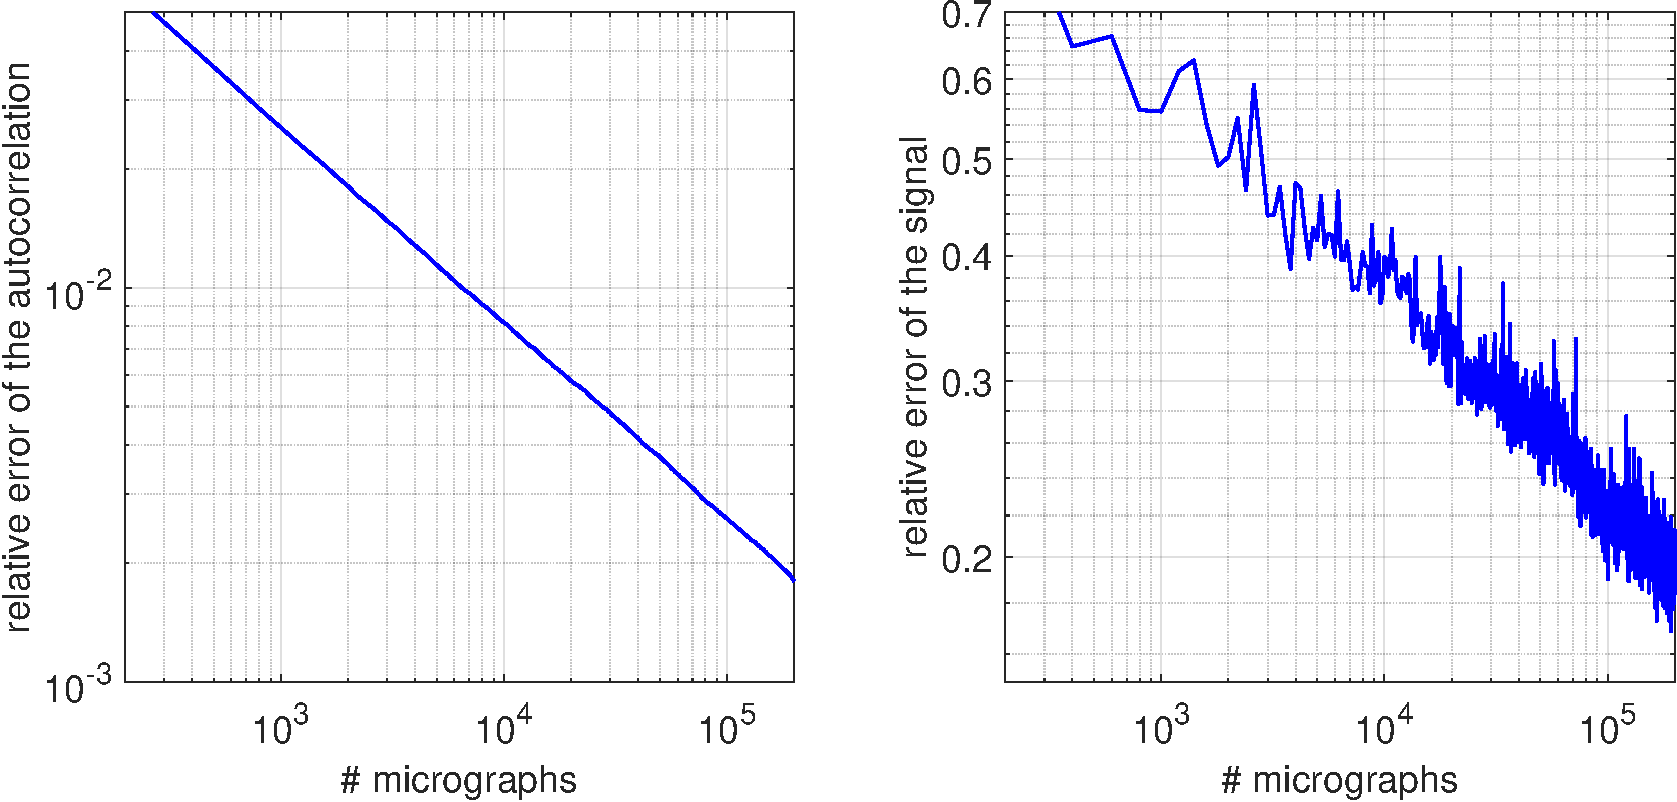
\includegraphics[width=.8\linewidth]{Einstein_recovery_error_combined}
%	\caption{\label{fig:error_per_micro}Relative error curves for the experiment of Figure~\ref{fig:Einst_example}.}
%\end{figure}
%
%
%In practice, we do not expect to know $\gamma$ and maybe not even $\sigma$.
%Figure~\ref{fig:1D_example} %(see appendix) 
%shows recovery of a 1-D signal from the first three autocorrelations of the data.
%The autocorrelations are computed from noisy micrographs with $\sigma=3$ that obey the separation condition of~\eqref{eq:spacing}; see Figure~\ref{fig:1D_obs_example}.  
%Both the signal  and $\gamma$ are estimated simultaneously from the observed autocorrelations by LS fitting; more details are given in Appendix~\ref{sec:numeric_details}. Crucially, the LS does not require  knowledge of $\sigma$. 
%
%
%\begin{figure}[h]
%	\centering
%	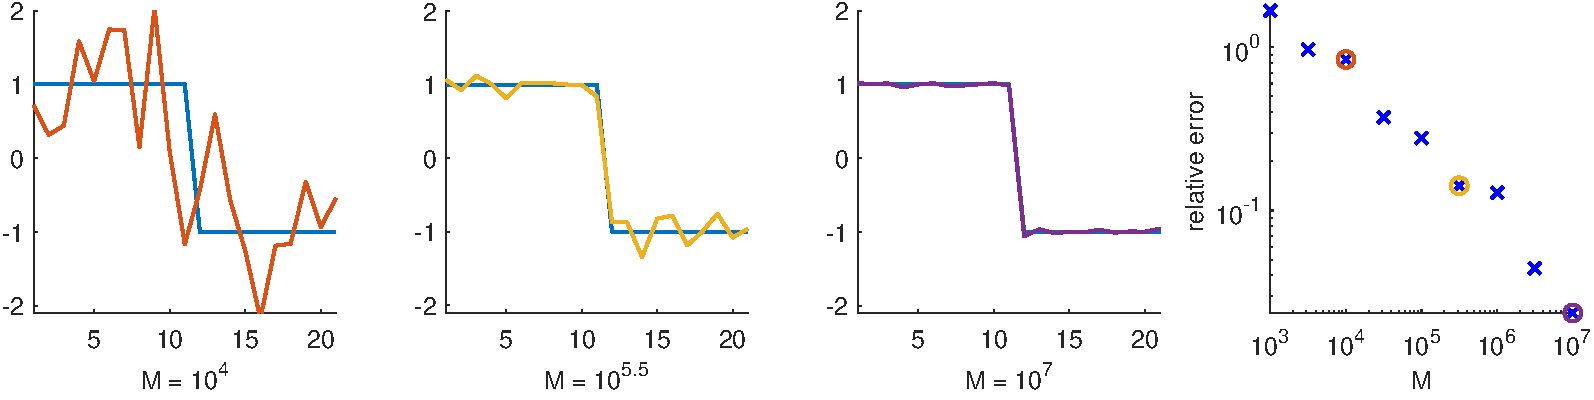
\includegraphics[width=\linewidth]{1D_example}
%	\caption{\label{fig:1D_example} Recovery of a 1-D signal of length $L=21$ at noise level $\sigma = 3$ from $M$ repetitions. The length of the micrograph was set to be $N = 410*M$. The first three panels (left to right) show reconstruction with different $M$ values compared to the ground truth signal (in blue).
%		The true value of $\gamma$ is $0.0512$.
%		The relative errors of $\gamma$ for the three panels are: $4.8\%,4\%,1.2\%$. The right panel shows the relative error as a function of $M$. 
%	}
%\end{figure}
%
%
%\begin{figure}[h]
%	\centering
%	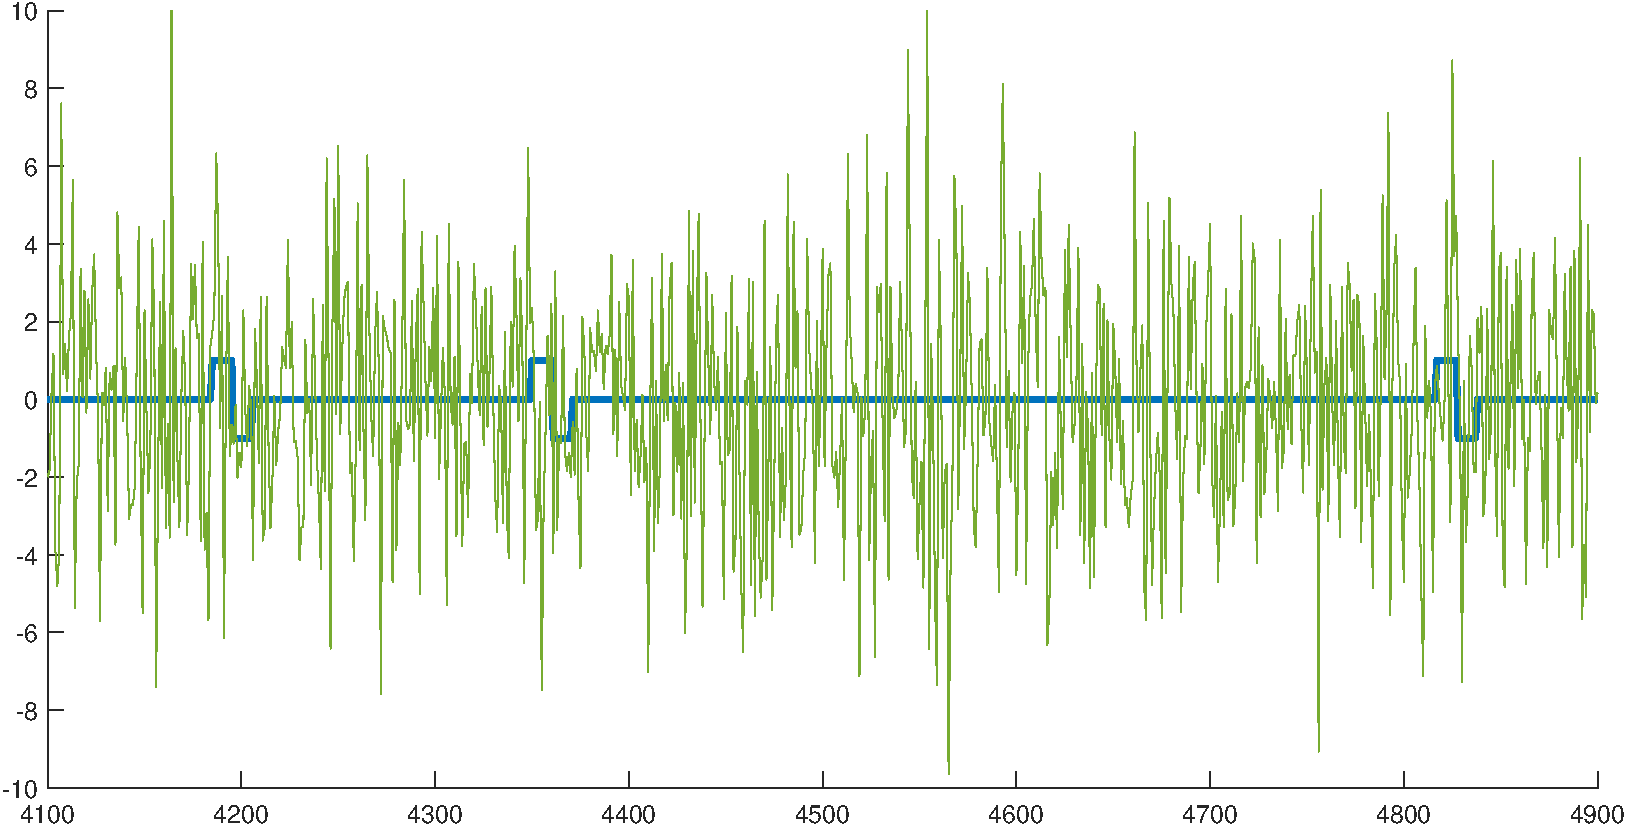
\includegraphics[width=0.6\linewidth]{example_obs_1D}
%	\caption{\label{fig:1D_obs_example} An example for a 1-D noisy measurement for the experiment in Figure~\ref{fig:1D_example}. The signal occurrences appear in blue, and the noisy data in green.
%	}
%\end{figure}
%
%
%\subsection{Cryo-EM} The application of autocorrelation analysis to cryo-EM follows the same mathematical principles.
%The derivation of the first three autocorrelations of the micrographs and their relations to the volume itself are provided in Appendix~\ref{sec:ac_cryo}.
%In particular, numerical evidence suggests that the third-order autocorrelation uniquely determines the 3-D volume. 
%Figure~\ref{fig:cryo_recon} shows recovery of the 3-D volume from the clean autocorrelations and from noisy micrographs. 
%Excerpts from the noisy micrographs are shown in Figure~\ref{fig:cryo_noisy_micros_for_rec}.
%Unfortunately, the mapping between the autocorrelations and volume seems to be ill-conditioned, preventing high-resolution recovery from noisy data.
%The details of the reconstruction algorithm are given in Appendix~\ref{sec:numeric_details}.
%In the next section, we outline how we suggest to overcome the ill-conditioning in future work. 
%
%\begin{figure}[h]
%	\centering
%	\begin{subfigure}[h]{0.45\textwidth}
%		\centering
%		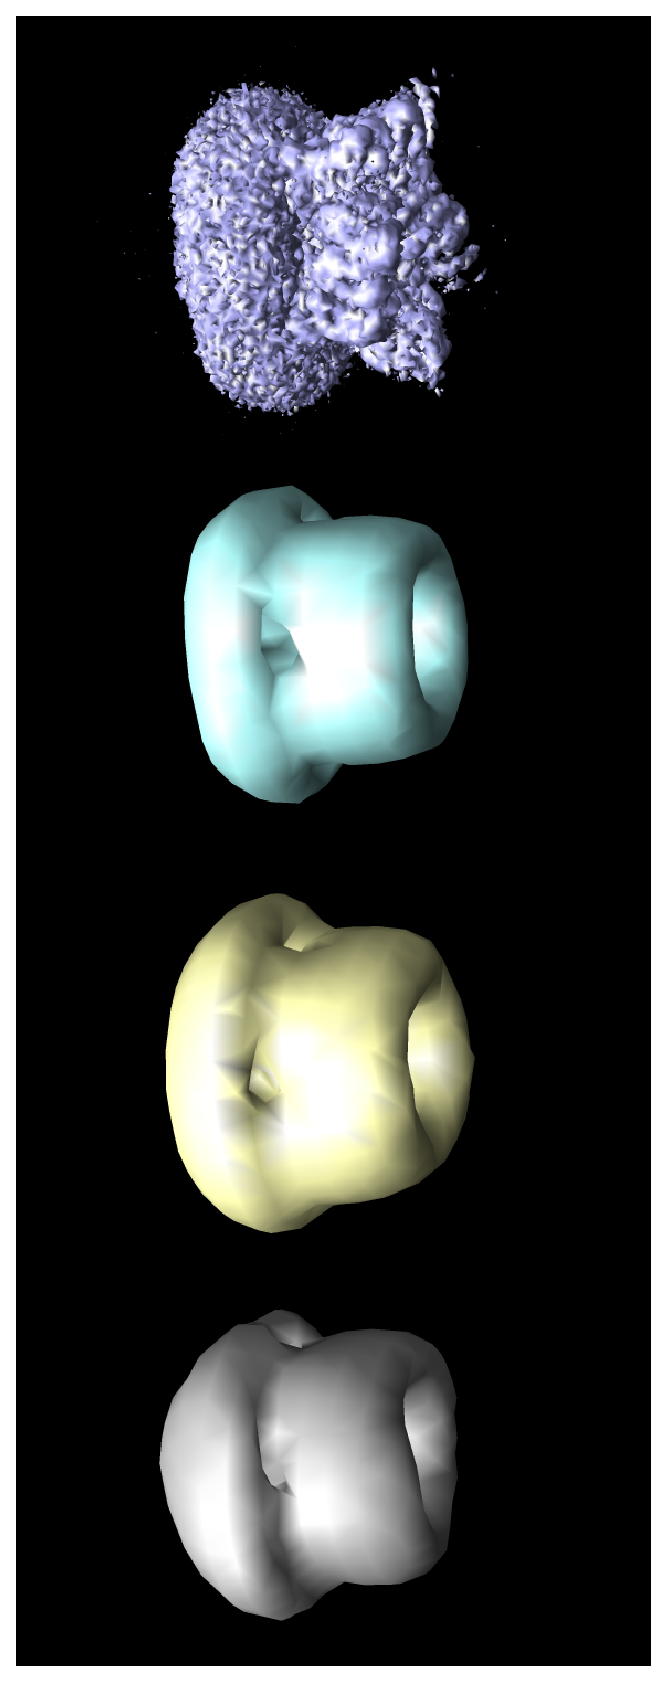
\includegraphics[angle=270, width=1\textwidth]{TRPV1_rec_incl_noisy_resize.eps}
%		\caption{TPRV1 with cutoff $L_{\text{max}}=5$}\label{fig:TRPV1_recon}
%	\end{subfigure}
%	\hfill
%	\begin{subfigure}[h]{0.45\textwidth}
%		\centering
%		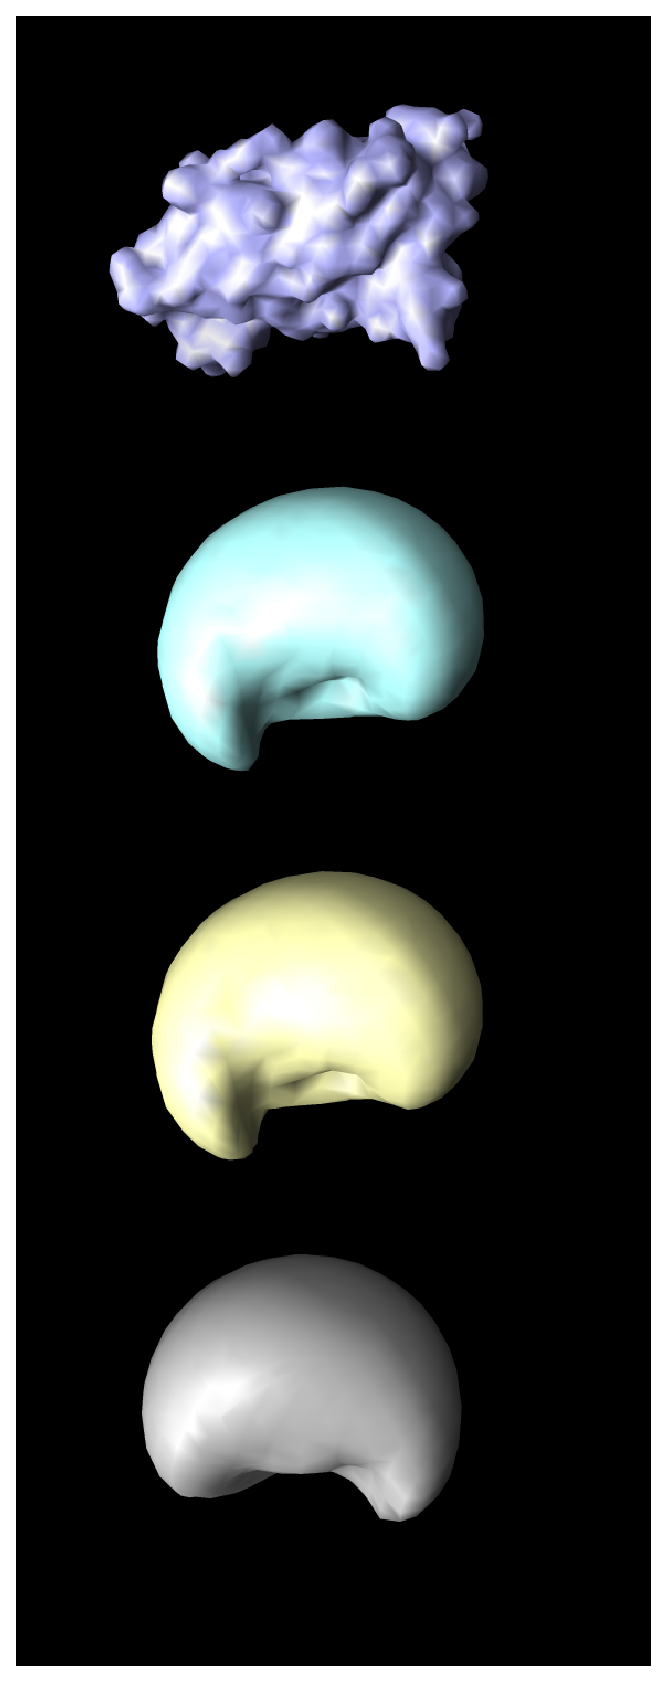
\includegraphics[angle=270, width=1\textwidth]{BPTI_maxL2_L20_resize.eps}
%		\caption{BPTI with cutoff $L_{\text{max}}=2$}\label{fig:BPTI_recon}
%	\end{subfigure} 
%	\caption{\label{fig:cryo_recon} Reconstructions from the first, second and third order autocorrelations.
%		The ground truth volumes were expanded according to~\eqref{eq:volume_expansion_app} with cutoff $L_{\text{max}}$.
%		{The original molecules are shown in purple and the (smoothed) ground truths in blue  to illustrate the smoothing effect of our downsampling and truncation of the spherical harmonics expansion.
%			The reconstructions  from clean autocorrelations are shown in yellow and recoveries from 
%			autocorrelations estimated from noisy data in gray. For the noisy experiments, we used 300 micrographs with SNRs of 1/16 for TRPV1 and 1/64 for BPTI. We present excerpts from noisy micrographs side-by-side with the corresponding clean ones in Figure~\ref{fig:cryo_noisy_micros_for_rec} (see appendix)}.}
%	%	\vspace{-20pt} 	
%\end{figure}
%
%\begin{figure}[t!]
%	\centering
%	\begin{subfigure}[t]{0.245\textwidth}
%		\centering
%		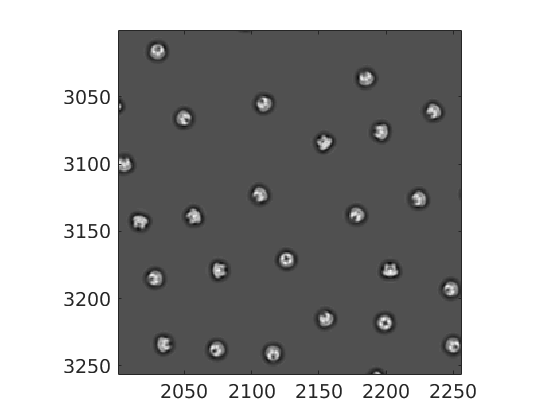
\includegraphics[scale=0.3]{TRPV1_clean_micro.png}
%		\caption{}
%	\end{subfigure} \hfill %\hspace{2pt}
%	\begin{subfigure}[t]{0.245\textwidth}
%		\centering
%		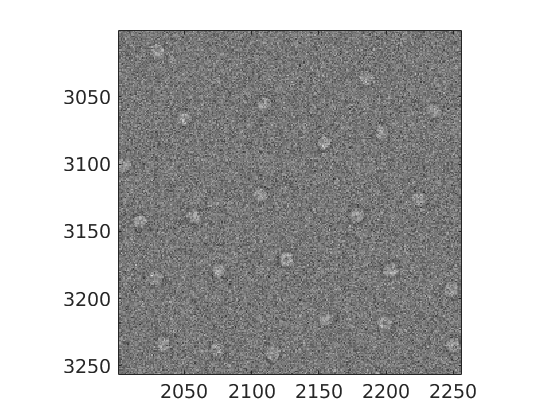
\includegraphics[scale=0.3]{TRPV1_noisy_micro_SNR_16.png}
%		\caption{}
%	\end{subfigure} \hfill %\hspace{2pt}
%	\begin{subfigure}[t]{0.245\textwidth}
%		\centering
%		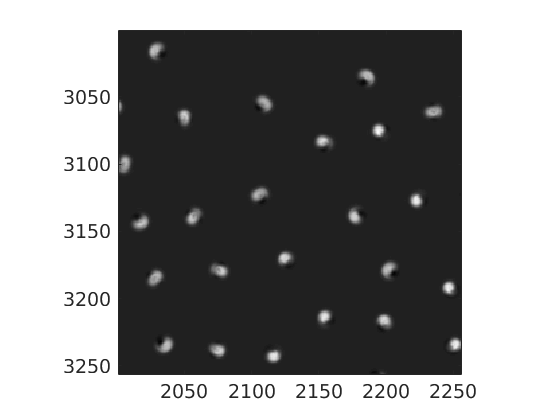
\includegraphics[scale=0.3]{clean_micro_BPTI.png}
%		\caption{}
%	\end{subfigure} \hfill
%	\begin{subfigure}[t]{0.245\textwidth}
%		\centering
%		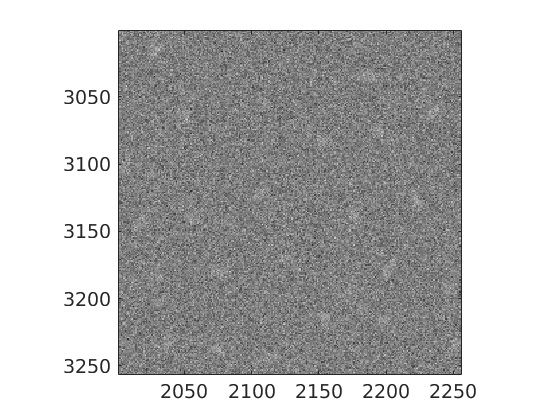
\includegraphics[scale=0.3]{noisy_micro_BPTI_SNR_64.png}
%		\caption{}
%	\end{subfigure}
%	\caption{\label{fig:cryo_noisy_micros_for_rec}  {Excerpts from the noisy micrographs used for the reconstructions in Figure~\ref{fig:cryo_recon} and the corresponding clean excerpts. (a) Excerpt of the clean TRPV1 micrograph; (b) Excerpt of the noisy TRPV1 micrograph with SNR $= 1/16$; (c) Excerpt from the clean BPTI micrograph; (d) Excerpt from the noisy BPTI micrograph with SNR $= 1/64$.}} 
%\end{figure}
%
%\begin{figure}[t!]
%	\centering
%	\begin{subfigure}[t]{0.4\textwidth}
%		\centering
%		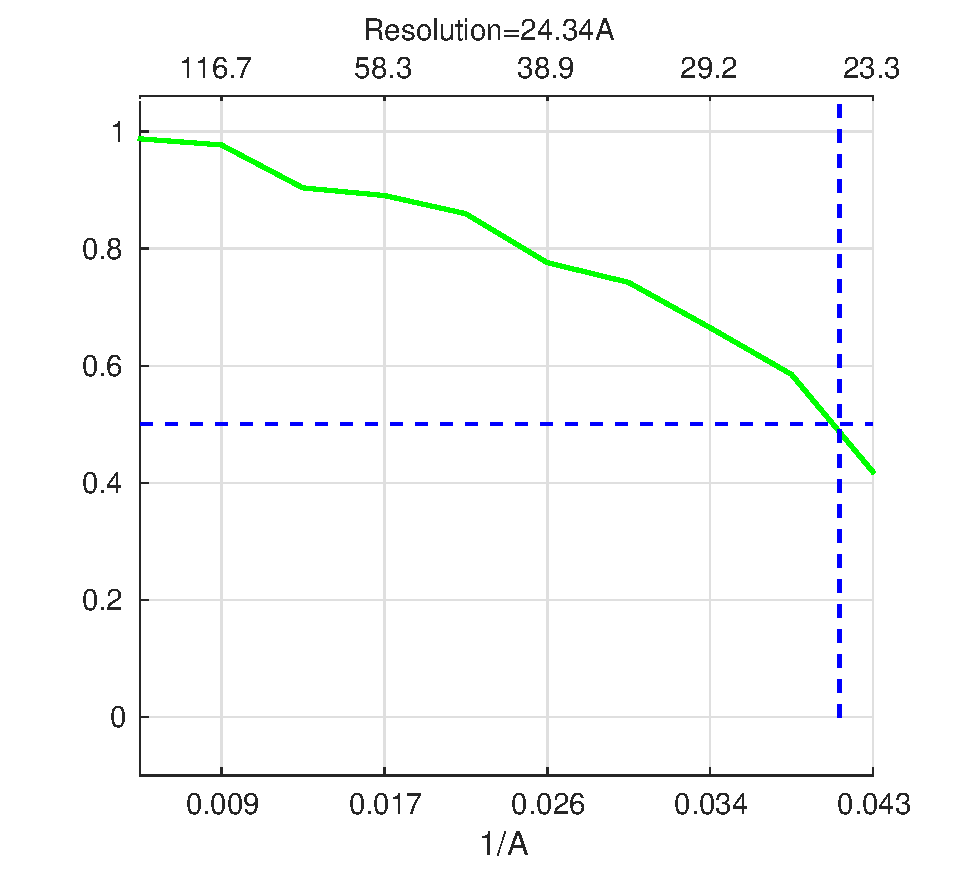
\includegraphics[scale=0.35]{TRPV1_trunc_FSC.eps}
%		\caption{}
%	\end{subfigure} \hfill %\hspace{2pt}
%	\begin{subfigure}[t]{0.4\textwidth}
%		\centering
%		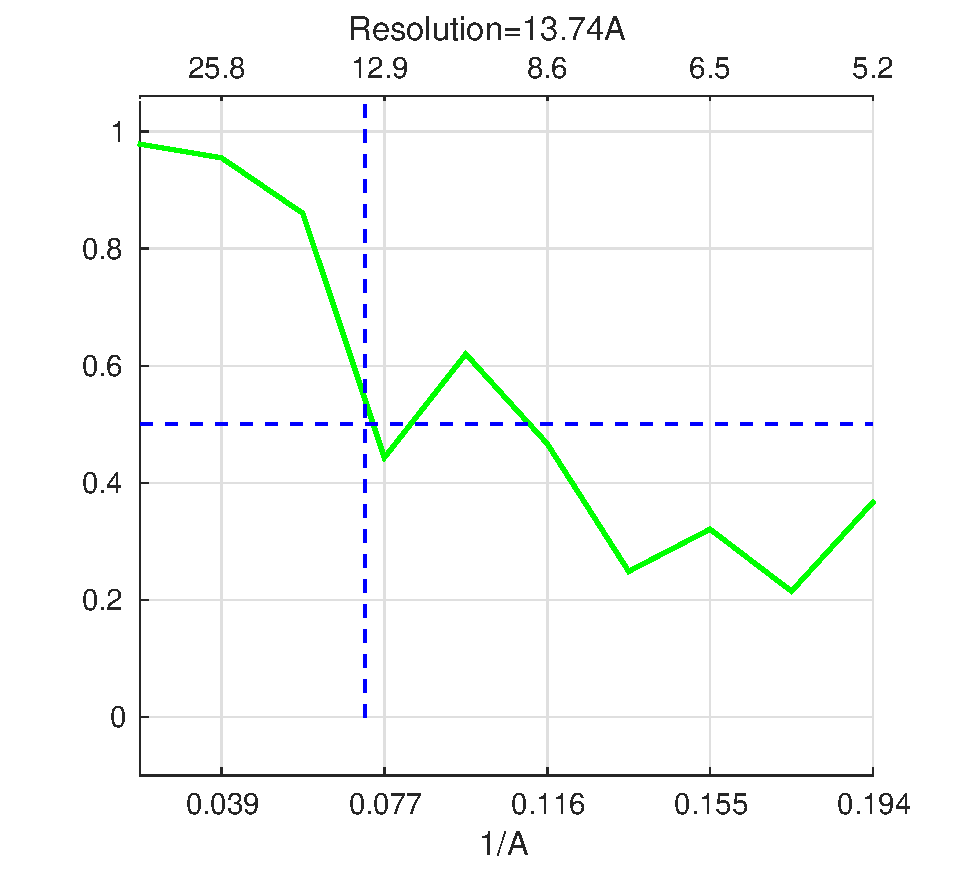
\includegraphics[scale=0.35]{BPTI_FSC.eps}
%		\caption{}
%	\end{subfigure} 
%	\caption{\label{fig:cryo_FSC}  {Fourier Shell Correlations (FSCs) for the noisy reconstructions presented in Figure~\ref{fig:cryo_recon} using the $0.5$ criterion, compared to the (smoothed) ground truth. (a) FSC for the TRPV1 reconstruction, giving resolution of $24$\AA; (b) FSC for the BPTI reconstruction, giving resolution of $13$\AA.}} 
%\end{figure}
%
%
%While we cannot provide a {high-resolution} 3-D reconstruction from noisy data with the current algorithm, our method can be easily applied to the problem of deciding whether a micrograph contains projections or merely pure noise---a problem considered in classical works in statistics~\cite{donoho2004higher} %and debates in the cryo-EM community~\cite{henderson2013avoiding}.
%and cryo-EM~\cite{henderson2013avoiding}.
%This task can be performed by considering solely the recovered $\gamma$ (the fraction of pixels occupied by projections in the micrograph), estimated as part of the recovery algorithm.
%Figure~\ref{fig:cryo_detection} %(see appendix) 
%presents excerpts  of two noisy micrographs, only one of which contains projections.
%In the presence of projections, the estimated $\gamma$ was $0.12$, corresponding to approximately $6784$ projections. 
%On the other hand, the estimated $\gamma$ drops to $10^{-5}$ for the pure noise micrograph, corresponding to less than one projection.
%
%
%\begin{figure}[h]
%	\centering
%	\begin{subfigure}[t]{0.3\textwidth}
%		\centering
%		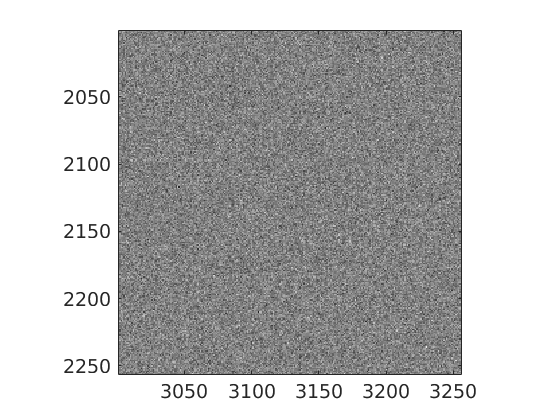
\includegraphics[scale=0.4]{pure_noise_micrograph_cutout.png}
%		\caption{An excerpt of the pure noise micrograph}
%	\end{subfigure} \hfill %\hspace{2pt}
%	\begin{subfigure}[t]{0.3\textwidth}
%		\centering
%		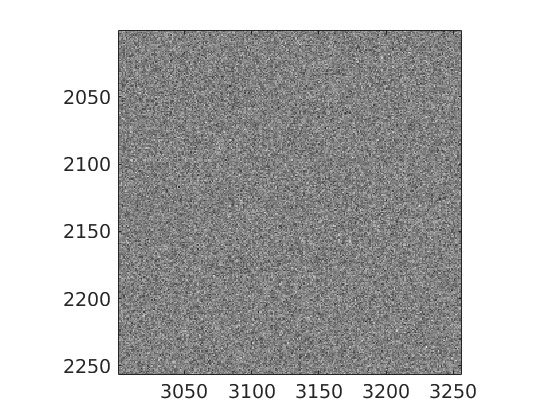
\includegraphics[scale=0.4]{noisy_micrograph_cutout.png}
%		\caption{An excerpt of the clean micrograph in right panel perturbed by the noise in the left panel.}
%	\end{subfigure} \hfill %\hspace{2pt}
%	\begin{subfigure}[t]{0.3\textwidth}
%		\centering
%		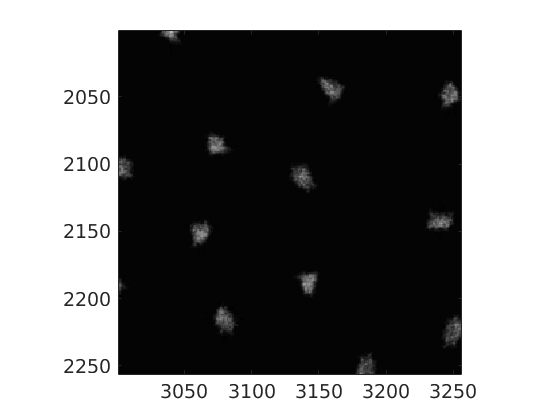
\includegraphics[scale=0.4]{clean_micrograph_cutout.png}
%		\caption{An excerpt of the clean micrograph}
%	\end{subfigure}
%	\caption{\label{fig:cryo_detection} All micrographs are of size $7420^2$ pixels and the projections are taken from the BPTI molecule of size $31^3$. The added noise was drawn from i.i.d.\ Gaussian distribution with zero mean and standard deviation $25$, corresponding to an SNR below $1/1024$.  
%		The noise realization is identical in both micrographs.} 
%\end{figure}


\section{Relation with cryo-EM + experiments?}
%
%In the simplified mathematical model above, we showed it is possible to estimate a signal without detecting its appearances.  
%Our strategy is to compute autocorrelations of the micrographs and to relate these statistics to the unknown signal's parameters. Recovering the parameters from the statistics reduces to solving a set of polynomial equations. 
%
%We also showed how this technique can, in principle, be applied to cryo-EM.
%Crucially, the outlined approach involves no particle picking, hence a fortiori no viewing direction estimation. Concerns for model bias are also greatly reduced since no template matching is involved.
%Additionally,  our technique also allows the use of much lower defocus values. Lower defocus means lower contrast, but will maintain  higher frequency information. Consequently, we may be able to get high resolution reconstructions from fewer micrographs.
%
%Looking toward applying the framework to encompass all important features of real cryo-EM experiments, our work implies that it might be possible to reconstruct small molecules, particularly, molecules that are too small to be detected in micrographs. 
%In pursuing this research direction, our goal is to significantly increase the range of molecules to which cryo-EM can be successfully applied.
%We recognize that significant challenges lay ahead for the implementation of the proposed approach to {high-resolution} 3-D reconstruction directly from the micrographs. We discuss a few now.
%
%The numerical experiments we have performed reveal that the third-order autocorrelation may not be enough for 3-D reconstruction in practice, due to high sensitivity.
%This suggests that fourth-order autocorrelation may be necessary. This in turn would imply that the procedure might require a large amount of data. 
%Recent trends in high-throughput cryo-EM technology   give hope that this may be a lesser concern in the long term. Still, large amounts of data also require large amounts of computation. On this front, we note that computing autocorrelations can be executed efficiently on CPUs and GPUs, and in parallel across micrographs. It can even be done in a  streaming mode, as only one pass through each micrograph is necessary. The output of this data processing stage is a summary in the form of autocorrelation estimates: its size is a function of the resolution, not a function of the number of observed micrographs. Subsequent steps, which involve solving the system of polynomial equations, scale only in the size of that summary. Of course, an important question then is whether the equations can be solved accurately and efficiently in practice. 
%
%To reach high-resolution reconstruction, beyond data acquisition and computational challenges, there are modeling issues  to consider.
%In contrast to the simplifying assumptions we have made above, the noise might be colored; the viewing directions of the particles may be distributed non-uniformly; there may be conformational heterogeneity; particles generally do not satisfy our separation condition; and micrographs undergo a contrast transfer function which we have omitted. All of these aspects can be handled with the same general strategy: establish a forward model relating the expected autocorrelations of the micrographs to the target volume(s) and all parameters necessary to model the above effects. 
%For instance, for colored noise, the forward model may involve multiple parameters to capture the power spectrum of the noise instead of the single parameter $\sigma^2$. 
%Similarly, instead of the separation condition, we can model the spacing between the projections using a parameterized pair-correlation function. Such a function models the distribution of distances between neighboring projections. The observed autocorrelations depend linearly on these parameters, which would be estimated as part of the inverse problem.
%All these aspects must be taken into account so the method can be applied on experimental data. We hope to take care of these issues in future research. 
%
%\section*{Acknowledgment}
%The authors  thank Ayelet Heimowitz, Joe Kileel,  Roy Lederman, Amit Moscovich, Nir Sharon and  Fred Sigworth for helpful discussions,  and Boris Landa and Yoel Shkolnisky for providing the code for the 2-D PSWFs expansion.
%The research was partially supported by Award Number R01GM090200 from the NIGMS, FA9550-17-1-0291 from AFOSR, Simons Foundation Math+X Investigator Award, and the Moore Foundation Data-Driven Discovery Investigator Award.
%NB is partially supported by NSF award DMS-1719558.

\bibliographystyle{plain}
\bibliography{ref}

\appendix

\section{Proof of Proposition~\ref{prop:gamma}} \label{sec:proof_prop_gamma}

In the limit, 
\begin{equation*}
(a^1_y)^2=\frac{\gamma^2}{L^2}\sum_{i=0}^{L-1}\sum_{j=0}^{L-1}x[i]x[j].
\end{equation*}
Similarly,  
\begin{equation*}
\sum_{\ell = 1}^{L-1}a_y^2[\ell]=\frac{\gamma}{L}\sum_{\ell = 1}^{L-1}\sum_{i=0}^{L-1-\ell}x[i]x[i+\ell],
\end{equation*}
and $a_y^2[0]=\frac{\gamma}{L}\sum_{i=0}^{L-1}x^2[i] + \sigma^2$. The proof is concluded by noting that  $a_x^2[-\ell]=a_x^2[\ell]$. 


\section{Proof of Proposition~\ref{prop:gamma_sigma}} \label{sec:proof_prop_gamma_sigma}

We prove that both $\sigma$ and $\gamma$ are identifiable from the observed first three moments of $y$. For convenience, we work with $\beta = \gamma / L$ rather than $\gamma$ itself. To this end, we construct two quadratic equations satisfied by $\beta$ and whose coefficients can be computed from observable quantities (in the limit). Then, we show that these equations are independent, and hence that $\beta$ is uniquely defined. Given $\beta$, we can estimate $\sigma$ using Proposition~\ref{prop:gamma}.

Throughout the proof, it is important to distinguish between observed and unobserved values.
We denote the observed values by $E_i$ or $a_y^1,a_y^2,a_y^3$. We use $F_i$ to denote functions of the signal's autocorrelations (which are not directly observable).

In the limit $N \to \infty$, almost surely, $a_y^1 = \beta(\one^Tx)$ and $a_y^2[0] = \beta\|x\|^2+\sigma^2$, where $\one\in\RL$ is the vector of all-ones. (In this whole section, for clarity, we now omit to specify that identities hold almost surely in the limit.) Consider the product:
\begin{equation}\label{eq:E1}
\begin{split}
E_1 := a_y^1a_y^2[0] =  (\beta(\one^Tx))(\beta\|x\|^2+\sigma^2)  = \sigma^2a_y^1 + L\beta^2F_1,
\end{split}
\end{equation}
where $F_1 := a_x^3[0,0] + \sum_{j=1}^{L-1}(a_x^3[j,j] + a_x^3[0,j])$. 
% Nicolas: the expression for F_1 is correct, see identifiability_of_gamma_and_sigma_Sep4_2018.m and notes Sep 4, 2018
The terms of $F_1$ can also be estimated from $a_y^3$, while taking the scaling and bias terms into account. This yields another observable:
\begin{align} 
E_2 & := a_y^3[0,0] + \sum_{j=1}^{L-1}(a_y^3[j,j] + a_y^3[0,j]) \nonumber\\
& = L\beta F_1 + (2L+1)\sigma^2a_y^1. \label{eq:E2}
\end{align}
% Nicolas: checked this one too.
Therefore, from~\eqref{eq:E1} and~\eqref{eq:E2} we get:
\begin{equation} \label{eq:E12}
E_2\beta -(2L+1)\sigma^2\beta a_y^1 = E_1-\sigma^2a_y^1.
\end{equation}
Let $E_3:=a_y^2[0] + 2\sum_{j = 1}^{L-1}a_y^2[j]$; recall from Proposition~\ref{prop:gamma}:
\begin{equation} \label{eq:sigma2}
\sigma^2 = E_3 - (a^1_y)^2/\beta. 
\end{equation} 
Plugging into~\eqref{eq:E12} and rearranging, we get a first quadratic equation in $\beta$,
\begin{equation} \label{eq:quad1}
\mathcal{A}\beta^2 + \mathcal{B}\beta + \mathcal{C} = 0,
\end{equation}
where 
\begin{align*}
\mathcal{A} &= E_2 - (2L+1)a_y^1E_3, \\ 
\mathcal{B} &= -E_1 + (2L+1)(a_y^1)^3 + a_y^1E_3  , \\
\mathcal{C} &= -(a_y^1)^3.
\end{align*}
Importantly, these coefficients are observable quantities. As we assume throughout this proof that $x$ has nonzero mean, $a_y^1 \neq 0$ and we conclude that this equation is non-trivial.

Next, we derive the second quadratic equation for $\beta$. We notice that 
\begin{equation} \label{eq:E3}
E_4 := \frac{1}{L}(a_y^1)^3 = \frac{1}{L}\beta^3 (\one ^Tx)^3   = \beta^3 F_2,
\end{equation}
where $F_2 = \frac{1}{L}(\one ^Tx)^3$, and we can work out that:
\begin{equation*}
F_2 = a_x^3[0,0] + 3\sum_{j=1}^{L-1} \left(a_x^3[j,j] + a_x^3[0,j]\right) + 6\sum_{1\leq i < j\leq L-1}a_x^3[i,j].
\end{equation*}
Once again, $F_2$ can be estimated from $a_y^3$, taking bias and scaling into account:
\begin{align}
E_5 & := a_y^3[0,0] + 3\sum_{j=1}^{L-1} \left(a_y^3[j,j] + a_y^3[0,j]\right) + 6\sum_{1\leq i < j\leq L-1}a_y^3[i,j]  = L \beta F_2 + (6L-3)\sigma^2a_y^1.
\end{align}
Consider the following ratio:
\begin{equation*} 
\frac{E_5}{E_4} = \frac{L}{\beta^2} + \frac{(6L-3)\sigma^2a_y^1}{E_4}.
\end{equation*}
From the latter, we deduce:
\begin{equation*}
\sigma^2 = \frac{E_5}{a_y^1(6L-3)}  - \frac{LE_4}{\beta^2a_y^1(6L-3)}.
\end{equation*}
Using~\eqref{eq:sigma2} and rearranging, we get the second quadratic:
\begin{equation} \label{eq:quad2}
\mathcal{D}\beta^2 + \mathcal{E}\beta + \mathcal{F} = 0,
\end{equation}
where
\begin{align*}
\mathcal{D} &= E_3 - \frac{E_5}{a_y^1(6L-3)}, \\ 
\mathcal{E} &= -(a_y^1)^2, \\
\mathcal{F} &= \frac{LE_4}{a_y^1(6L-3)}.
\end{align*}
It is also non-trivial since $E_4 \neq 0$.

To complete the proof, we need to show that the two quadratic equations~\eqref{eq:quad1} and~\eqref{eq:quad2} are independent. To this end, it is enough to show that the ratios between coefficients differ. 
From~\eqref{eq:quad1} and~\eqref{eq:E1}, we have:
\begin{equation*}
\begin{split}
\frac{\mathcal{B}}{\mathcal{C}} = \frac{E_1 - (2L+1)(a_y^1)^3 - a_y^1E_3}{(a_y^1)^3} = \frac{a_y^2[0] - (2L+1)(a_y^1)^2 - E_3}{(a_y^1)^2}.
\end{split}
\end{equation*}
In addition, using~\eqref{eq:E3},
\begin{equation*}
\frac{\mathcal{E}}{\mathcal{F}} = \frac{(3-6L)(a_y^1)^3}{LE_4} = 3 - 6L . 
\end{equation*}
For contradiction, suppose that the quadratics are dependent. Then, $\frac{\mathcal{B}}{\mathcal{C}} =\frac{\mathcal{E}}{\mathcal{F}} $, that is, 	
\begin{equation*}
a_y^2[0] - (2L+1)(a_y^1)^2 - E_3 = (a_y^1)^2(3-6L).
\end{equation*}
Rewriting the identity in terms of $x$ and dividing by $\beta$ we get:
\begin{equation} \label{eq:cond}
4(L-1)\beta (\1^\top x)^2  - (\1^\top x)^2 + \|x\|^2 = 0.
\end{equation}	
For generic $x$,  this polynomial equation is not satisfied so that the quadratic equations are independent. 
Furthermore, from the inequality $L\|x\|^2 \ge (\1^\top x)^2$ it follows immediately that the equations must be independent so long as
\begin{equation*}
\beta > \frac{1}{4L}.
\end{equation*}

\end{document}


